% !TEX root = DataDrivenBayes.tex

\section{Case study 1: Focusing on optimality does not always lead to the best understanding of human behavior}

Our first case study revisits the Bayesian theory of coincidences and discoveries developed by \citeA[henceforth GT1]{Griffiths2007}. The central goal in that paper was to develop a Bayesian account of how people decide whether a pattern of observations is a mere coincidence (a chance occurrence) and when it represents a meaningful discovery. The paper uses Bayesian models to make normative claims. For instance, the abstract of the paper argues ``that people can {\it accurately} assess the strength of coincidences, suggesting that {\it irrational conclusions} drawn from coincidences are the consequence of overestimation of the plausibility of novel causal forces'', and on page 218 the authors argue that  ``human {\it irrationality} concerning coincidences [can] be localized in miscalibrated prior odds'' (emphasis ours). The normative claims are clear: To agree with this model is to be accurate and rational, and disagreements with the model are irrational. Moreover, to the extent that discussion of the Bayesian theory focuses on such claims, the purpose of constructing the Bayesian model appears to be that it licenses these normative claims. 

In this case study we focus on two problems that sometimes arise when applying the optimal Bayesian approach. First, demonstrating that aggregated response curves match those produced by an optimal model may not provide sufficient evidence that people's behavior is optimal if {\it individual} responses deviate from the optimal norm. Second, when behavior cannot reasonably be considered to be optimal, this type of model loses its explanatory power and provides limited psychological insights. We address these issues by including a descriptive Bayesian model in our analysis---one that best describes human behavior and drops any normative claims about the rationality of human cognition---and show that this leads to additional insights about human psychology, including a more nuanced understanding of how people's behavior deviates from optimality.


\subsection{Of genetics and psychokinetics: Inference from binary data}

The original GT1 paper discusses several different inference problems and develops a Bayesian model for each one, but for our purposes it will be sufficient to consider the simplest case. In their first experiment, they presented people with descriptions of fictitious scientific experiments in which the observed outcomes were binary, and the question people had to answer was whether the true base rate of the outcomes was 50\%. There were two versions of the task. People in the {\sc genetics} condition were given the following cover story:

\begin{quote}
{\it A group of scientists investigating genetic engineering have conducted a series of experiments testing drugs that influence the development of rat fetuses. All of these drugs are supposed to affect the sex chromosome: they are intended to affect whether rats are born male or female. The scientists tested this claim by producing 100 baby rats from mothers treated with the drugs. Under normal circumstances, male and female rats are equally likely to be born. The results of these experiments are shown below: The identities of the drugs are concealed with numbers, but you are given the number of times male or female rats were produced by mothers treated with each drug.}
\end{quote}

\noindent
After being told that (say) 70 out of the 100 baby rats were male, participants were asked to assess the probability that the drug was effective. In a classical null hypothesis test, the inferences that one makes in this scenario depend only on the raw data (i.e., number of males and number of females). However, GT1 argue that people should treat this as Bayesian inference problem and use the cover story to impose some prior bias. To that end, a second group of participants (in the {\sc psychokinesis} condition) saw this cover story:

\begin{quote}
{\it A group of scientists investigating paranormal phenomena have conducted a series of experiments testing people who claim to possess psychic powers. All of these people say that they have psychokinetic abilities: They believe that they can influence the outcome of a coin toss. The scientists tested this claim by flipping a fair coin 100 times in front of each person as they focus their psychic energies. Under normal circumstances, a fair coin produces heads and tails with equal probability. The results of these experiments are shown below: The identities of the people are concealed with subject numbers, but you are given the number of times the coin came up heads or tails while that person was focusing their psychic energies.}
\end{quote}

Participants were then shown the outcomes of a series of these experiments---the number of male rats or the number of heads out 100 trials---and had to judge the probability that the drug affected the sex of rats, or that the person had psychic powers. In order examine how people's beliefs are the strength of evidence in the data, they asked people to judge the probability that the drug/psychokinesis was effective in 8 different situations: when the number of males/heads was 47, 51, 55, 59, 63, 70, 87, 99 and 100. 


\subsection*{An optimal Bayesian model}

How should an optimal reasoner behave when solving this problem? GT1 present the following rational analysis of the task. There are two hypotheses that need to be discriminated: According to the ``null'' hypothesis $h_0$, the true probability of male/heads is fixed at 50\%, but according to the ``alternative'' hypothesis $h_1$ the true probability is an unknown value $\theta$ that could be anywhere between 0 and 1. This framing of the problem seems entirely reasonable and in fact this exact model is sometimes used as a simple data analysis tool \cite<e.g.,>{wagenmakers_practical_2007}. Formally, if $n$ denotes the number of observations and $k$ denotes the number of successes, then the strength of evidence provided by the data is provided by the Bayes factor:
\begin{equation}\label{eq:gt1-likelihood}
\dfrac{P(\bm{x} \mid h_1)}{P(\bm{x} \mid h_0)} = \dfrac{2^n}{\tbinom{n}{k}(n+1)}
\end{equation}
The further that the proportion $k/n$ deviates from 0.5, the stronger the evidence for the alternative model. However, there are good reasons to think that people would be more skeptical of a claim about psychic powers than a claim about genetic engineering, and so GT1 argue that people should employ different priors in the two conditions. This also seems sensible, and similar claims about the importance of adapting the prior to suite the problem have been made in the Bayesian data analysis literature \cite{wagenmakers_why_2011}. Multiplying the Bayes factor by the prior odds $P(h_1)/P(h_0)$ gives us the posterior odds ratio, 
\begin{equation}\label{eq:gt1-posterior}
\dfrac{P(h_1 \mid \bm{x})}{P(h_0  \mid \bm{x})} = \dfrac{P(\bm{x} \mid h_1)}{P(\bm{x} \mid h_0)} \times \dfrac{P(h_1)}{P(h_0)}
\end{equation}
which reflects the relative strength of belief that the learner has in the two hypotheses after the data have been observed.

The optimal model developed by GT1 is elegant, simple and makes very clear predictions about how different experimental manipulations should change people's judgments. The cover story manipulation should shape people's priors $P(h)$, the number of observed cases should affect the likelihood $P(x|h)$, and these two factors should be integrated via Bayes' rule. In light of the way in which they constructed their task and presented it to participants, we would strongly agree with their claim that this model does make sense as a normative standard for this task.

\subsection*{Successes and failures of the optimal model: A replication of the GT1 study}

How plausible is the claim that people are optimal at this task? To evaluate the optimal Bayesian model as a theory of human behavior, we conducted a replication of the GT1 experiment using 102 participants recruited through Amazon Mechanical Turk. Participants were paid \$0.40 for completing the study. The only difference between our study and the original one is that we used a slightly different dependent measure: We asked people to judge the probability that a real effect was observed. Following GT1, we excluded participants who appeared to have reversed the response scale (i.e., showed decreasing confidence in an effect as $k$ increased), leaving 89 participants. The results of the original study and our replication are shown as the solid lines in in Figure~\ref{fig:aggregate}. As is immediately clear from inspection of the figure, the empirical result from GT1 replicates.

\begin{figure}[!t]
	\centering
	(a) \\
	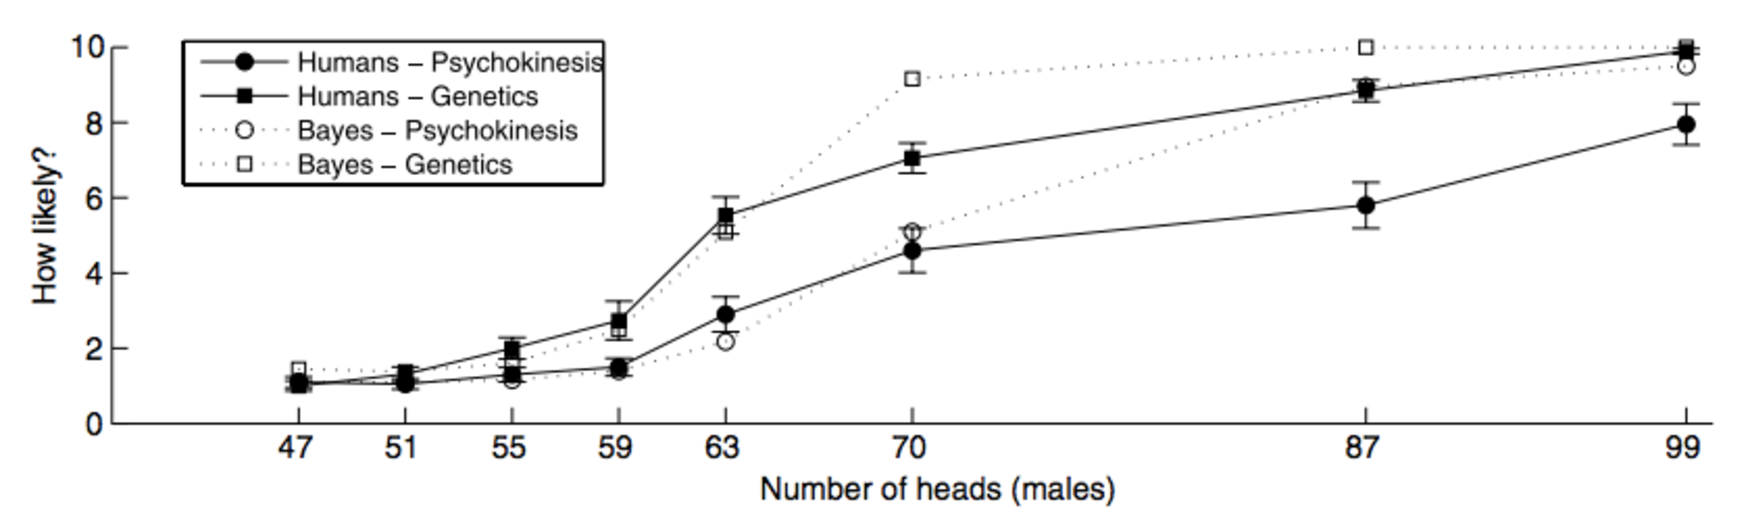
\includegraphics[width=0.7\textwidth]{coincidences_figures/gt1aggregate.pdf} \\
	(b) \\
	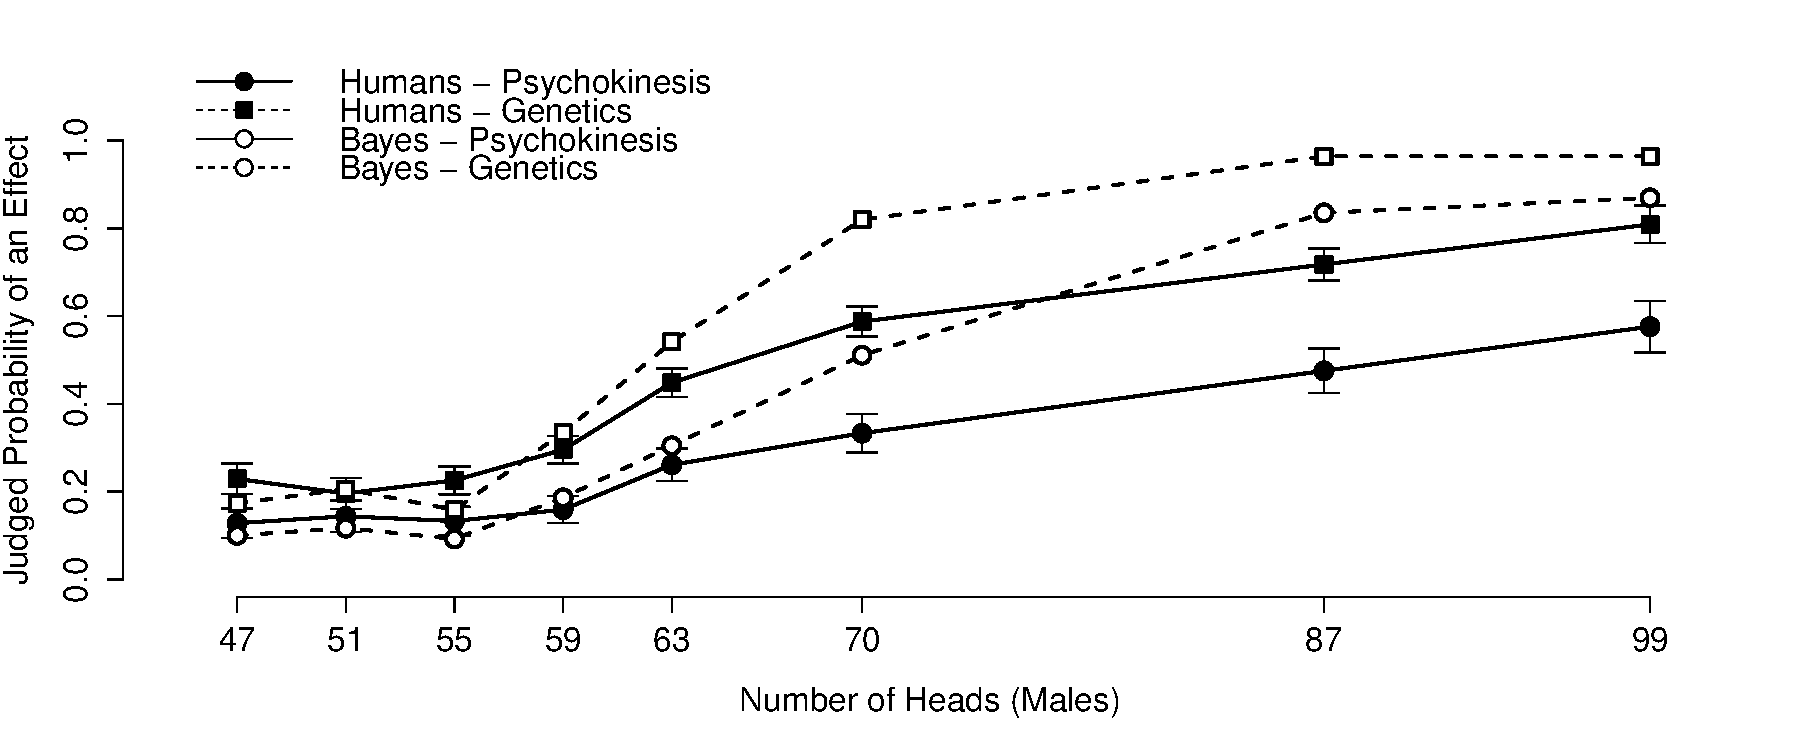
\includegraphics[width=0.75\textwidth]{coincidences_figures/usaggregate.pdf} \\
	\caption{Aggregated fits of the original Bayesian coincidences model. Panel (a) is a reproduction of Figure 3 from \protect\citeA{Griffiths2007}, whereas panel (b) shows the results from our replication of the experiment and model fitting procedure from the original paper. Error bars in panel (b) are standard errors. While there are some differences between the two panels, and some disagreements between the Bayesian model and human performance, the overall qualitative agreement is reasonable.}
	\label{fig:aggregate}
\end{figure}

In addition to replicating the experiment itself, we replicated the data analysis reported by GT1. When considering the application of the optimal model to empirical data, GT1 quite sensibly acknowledge that their Bayesian model allows room for some individual differences. As they note, it is reasonable to think that different people could read the same cover story and apply somewhat different priors. To accommodate this, they estimate a single free parameter (the prior odds) for each participant, and then reported the averaged responses for both model and humans.\footnote{A minor point on the model fitting exercise: the GT1 paper does not state what procedure was used to estimate parameters, though when fitting the data from our replication we found that minimizing sum squared error worked well. There is also a slight ambiguity in the way in which GT1 describe their procedure, insofar as the text refers to ``fitting the sigmoid function'' (their Equation 6), but also state that the parameters of the relevant sigmoid were fixed to have gain 1 and bias 0. On our reading of the text, it appears that this is intended to mean that the only free parameter in the model is the prior $P(h_1$), and that the sigmoid referred to in the relevant passage is intended only to ensure that $P(\mbox{effect}|\bm{x}) = P(h_1 | \bm{x})$.} These aggregated curves are plotted in Figure~\ref{fig:aggregate} and it is again clear that our replication of the data analysis is in agreement with the results in GT1. In both figures it is clear that the averaged model fits are a reasonable approximation to the averaged data, though clearly there are some fairly noticeable deviations too. 

\subsection{A closer look at the individual differences}

Figure~\ref{fig:aggregate} presents a single clean picture, one in which there is one pattern of performance produced by humans, and another single pattern produced by an optimal Bayesian reasoner. The fact that these two curves are in agreement (at least qualitatively) does make it look like people are doing optimal inference. Yet one is compelled to wonder: Do the responses of individual subjects look anything like these aggregated curves? Do individual subjects rely on a likelihood function based on independent Bernoulli trials? Should we call their reasoning be ``irrational'' if they do not? 

Viewed in this fashion, it is difficult to assess GT1's proposal that people behave optimally with respect to their prior: Their analysis acknowledges that individual differences might exist and estimates model parameters at the individual subject level, yet ultimately the model performance is assessed only in terms of the aggregated data.\footnote{We do not intend to single out these particular authors on this point. Averaging is a common practice that has often been criticized in the data analysis literature \cite<e.g.,>{Lee2005,Navarro2006}, and there are many well-documented examples in which averaging systematically distorts the structure of the data \cite<e.g.,>{estes_problem_1956,heathcote_power_2000}. It is not a failing unique to Bayesian cognitive models.} In light of these concerns, Figure~\ref{fig:nonoptimal} plots the responses at an individual subject level (right panel), and contrasts these individual subject curves with the response curves produced by the optimal Bayesian model under different choices of the prior odds parameter (left panel). As is immediately obvious from inspection, there is a major mismatch between the two. The curves produced by the Bayesian model are extremely steep,\footnote{It is worth noting that the shallower curves produced by the model at an aggregate level (i.e. in Figure~\protect\ref{fig:aggregate}) are purely an averaging artifact. The original Bayesian analysis reported by GT1 {\it cannot} produce shallow response curves for individual subjects.} whereas almost all the empirical curves are quite shallow. Even before attempting to quantify model performance (see below), it is clear the optimal Bayesian model does not provide a good account of human behavior at an individual subject level. Absent any evidence that human behavior matches the model predictions, it is difficult to substantiate any claim about the optimality of human performance in this task. On the contrary, when measured against the standard that GT1 proposed---optimal belief revision with respect to a prior that can vary from person to person---human cognition appears to be decidely suboptimal.


\begin{figure}[t]
	\centering
	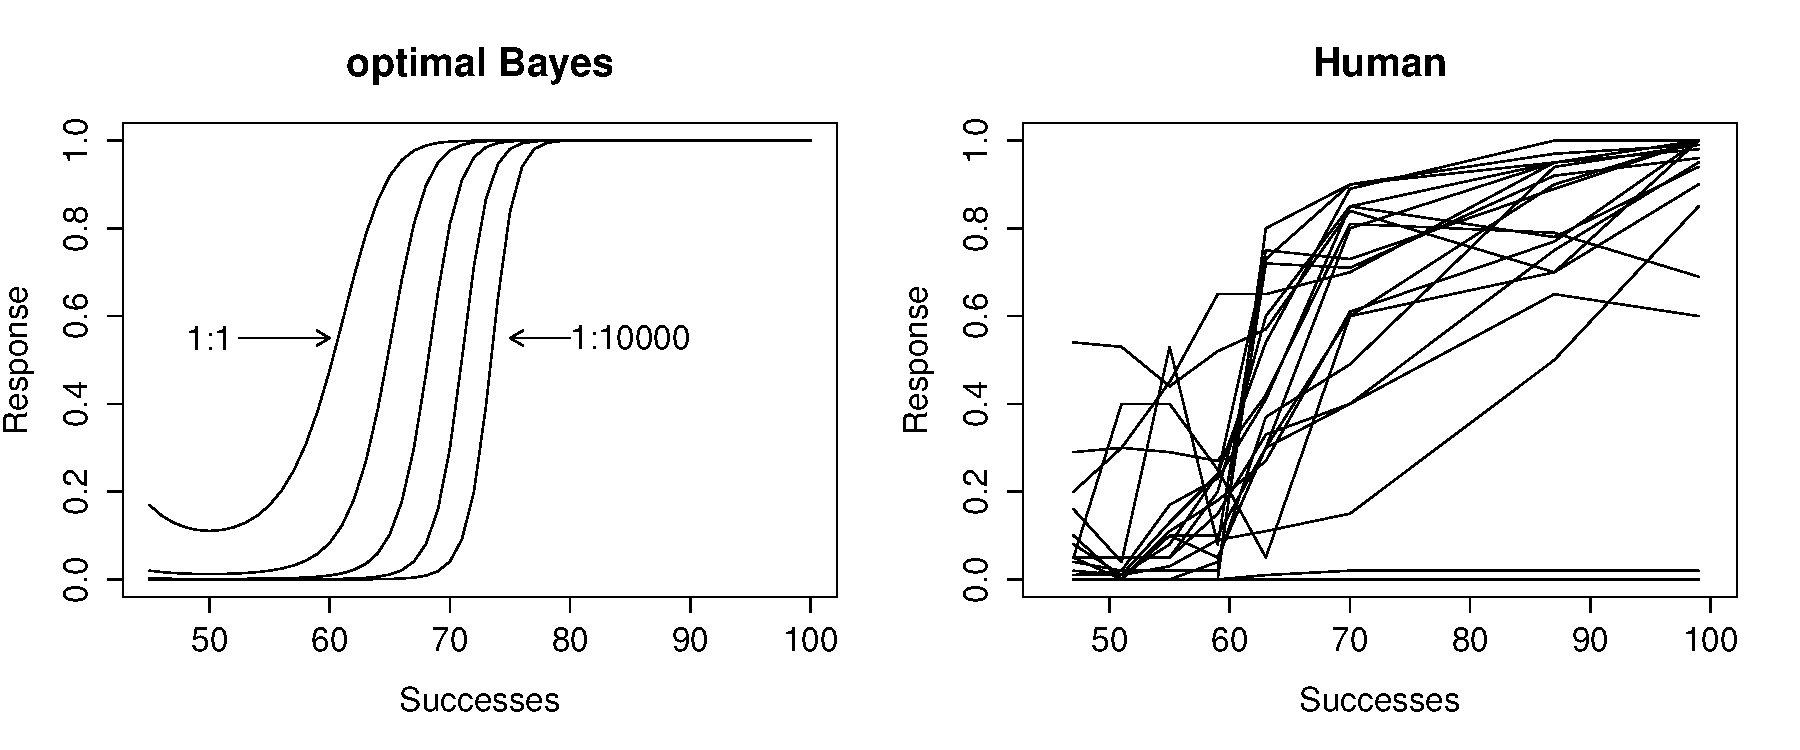
\includegraphics[width=1\textwidth]{coincidences_figures/nonoptimal.pdf}
	\caption{Systematic failures of the optimal Bayesian model for the coincidences task. The left panel plots the response curves predicted by the Bayesian model across a range of possible prior odds. For all choices of priors, the response curves are {\it extremely} steep, much moreso than the averaged curves plotted in Figure~\protect\ref{fig:aggregate}. In contrast, the right panel shows the response curves produced by 20 individual subjects, almost all of which are much shallower. }
	\label{fig:nonoptimal}
\end{figure}



\subsection*{A descriptive approach to the problem}

Given that the normative model proposed by GT1 does not provide a good account of the data, one might be tempted to conclude that we have exhausted the value of Bayesian cognitive models of this problem. Having shown that human performance is not optimal, perhaps we are now obligated to discard the Bayesian approach and turn to non-Bayesian accounts of human performance? We argue that this need not be true. In this section we present a descriptive Bayesian account of the same inference problem, and show that this approach sheds light on human performance even though we cannot use this model to justify any claim that the behavior it describes is rational, optimal or even appropriate. 

To construct our model, we begin by dropping GT1s claim that people integrate prior knowledge and statistical evidence in an ``appropriate'' fashion. Instead of requiring that our model use the Bernoulli likelihood function that a statistician might use to analyze scientific experiments, we allow specify a broad family of likelihood functions and seek to {\it learn} which ones produce human-like behavior. These likelihood functions may be appropriate to some real world problem that people have to solve, or they may not. Our initial goal is exploratory: Instead of using the Bayesian analysis as a tool to make claims about the optimality or appropriateness of people's responses, we treat it as a descriptive tool that helps us interpret the experimental data. From this descriptive perspective, it seems natural to want to explore the nature of individual differences and give them more prominence in the data analysis. 

With these goals in mind, we extend the model from GT1 in the following ways. Like GT1, we assume that people might have different priors. Letting $\phi = \log P(h_1)/P(h_0)$ denote the prior log odds, we approach the statistical inference problem as Bayesian data analysts and place a prior over $\phi$. More importantly, since we are giving up on the claim that people are necessarily adhering to an easily-definable standard of ``optimality'', we can take line of reasoning one step further. Why should people differ in their priors but not also their likelihoods? Assuming that everyone has the same likelihood function, as expressed in Equation~\ref{eq:gt1-likelihood}, makes sense if all people update their beliefs ``optimally'' (i.e., based on the assumption that each observation is the result of an independent Bernoulli trial). This is indeed what statistical models for binary data typically assume, but that does not mean that people make the same assumption. In many tasks people appear to update their beliefs conservatively \cite{phillips_conservatism_1966}, increasing their confidence in a proposition more slowly than the statistical evidence would warrant.

Incorporating conservatism into the GT1 model is not technically difficult. For example, a simple way to behave conservatively in this task is for the learner to apply Equation~\ref{eq:gt1-likelihood} to a smaller ``effective'' sample size than the one actually observed. Formally, we let $\theta$ denote the effective value of a single datum (ranging from 0 to 1), where each value of $\theta$ corresponds to a different likelihood function, and we obtain the original model from GT1 when $\theta=1$ \cite<see also>{navarro2012,RansomINPRESS}. Then, in the same way that we assume that people can have different priors $\phi$, we allow the possibility that each person has their own likelihood function defined by $\theta$. Then, adopting a Bayesian data analysis perspective, we as researchers specify our priors over the model parameters $\phi$ and $\theta$ and allow the empirical data to teach us something about our participants (see Appendix A for details). 

An important point to recognize is that while our expanded model is clearly {\it Bayesian}, it is difficult to characterize as an {\it optimal} model for the task that people were asked to solve. If participants do turn out to be conservative in their inferences, for intance, it is not at all obvious whether this conservatism has any normative justification. It is of course possible to construct post hoc stories about why it might be justified: One might argue that real world data are messy and autocorrelated, and as such it would be rational to display some conservatism if people transfer those expectations to the GT1 task. But even if this explanation were correct how much conservatism would real world messiness justify? It is not clear that there is a unique solution to this question. If our scientific goal is to judge whether people are doing the ``right thing'' or the ``wrong thing'', adding conservatism to the model seems to do nothing but muddy the waters. On the other hand, if we adopt the more exploratory goal of trying to find the statistical model that best describes human behavior, the focus shifts to empirical questions. What likelihoods and priors produce human-like behavior? Do they differ from person to person? Do they differ from context to context? These are questions we can investigate within the descriptive Bayesian framework, using the model as a tool, without being obligated to endorse any claim that the behavior that the model describes is optimal in any interesting sense of the word.

\begin{figure}[p]
	\centering
	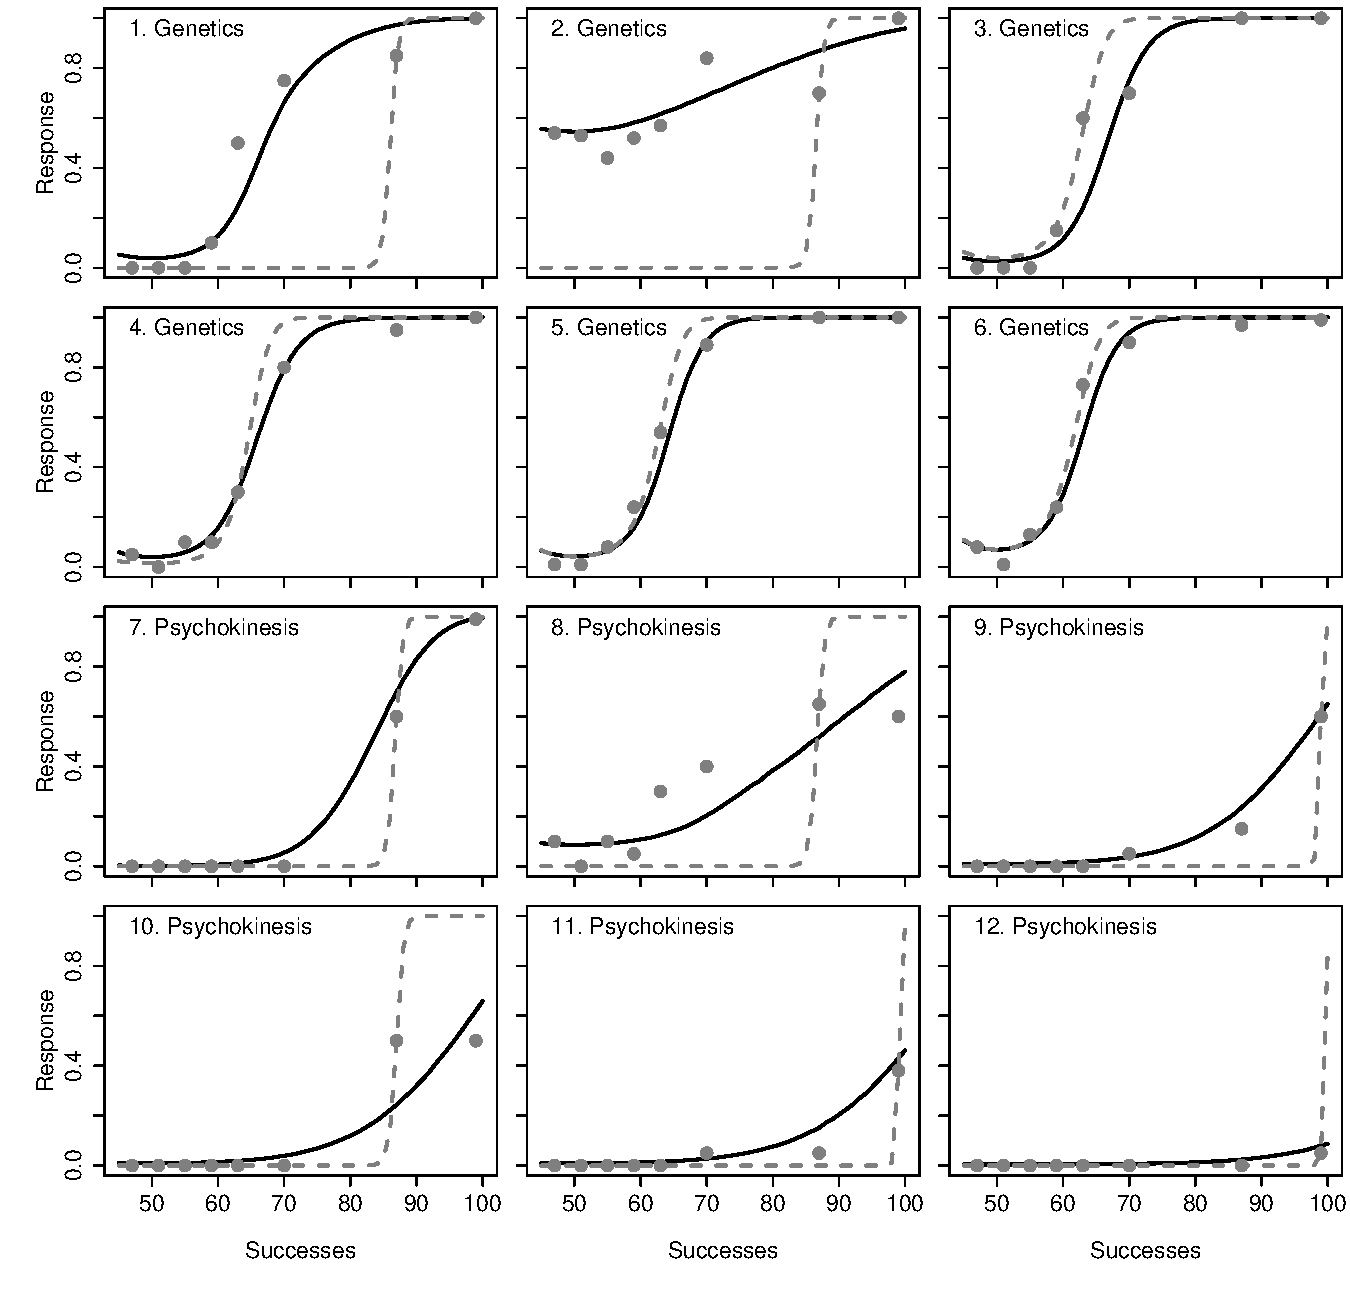
\includegraphics[width=1\textwidth]{coincidences_figures/individuals.pdf}
	\caption{Individual differences in the coincidences task. Each panel plots the responses from a single participant (dots). The top six panels show participants assigned to the {\sc genetics} condition and the bottom six panels show participants in the {\sc psychokinesis} condition.
Solid lines show the posterior predictive mean for the descriptive Bayesian model. Dotted lines show the fitted values for the original, optimal Bayesian model. It is clear that while the original model produces reasonable fits in some cases, in others (e.g., panels 1, 2, 8, 9, and 10) it performs much more poorly than the descriptive model. This is because it does not allow for any flexibility in the likelihood function, predicting a very steep rise as a function of the input.}
	\label{fig:indiv}
\end{figure}


\subsection*{Results}

\subsubsection*{The descriptive Bayesian model captures individual response curves}

Figure~\ref{fig:indiv} plots the raw data for twelve participants. In these plots, the dashed line shows the best fitting response curves for the original Bayesian model proposed by GT1, and the solid lines show the curves produced by the descriptive model. As is evident from inspection, there are some subjects who produce response curves that are in close agreement with the optimal Bayesian model. However, it is also evident that the optimal model only captures one possible human-like response pattern. In contrast, our expanded model provides reasonably good fits to all participants shown in Figure~\ref{fig:indiv}. For those participants who produce steep response curves, our model agrees with the original GT1 model. But the descriptive model can capture the behavior of people who produce shallower curves. As a result, by virtue of allowing a wider range of likelihood functions, our model passes a basic test of descriptive adequacy that the GT1 model fails. This is reflected in the average sum squared error between the model fits and the human data at the individual subject level: For the GT1 model it was 0.41 (sd = 0.45), whereas for the descriptive model it was 0.10 (sd = 0.14). 

\bigskip

\begin{figure}[]
	\centering
	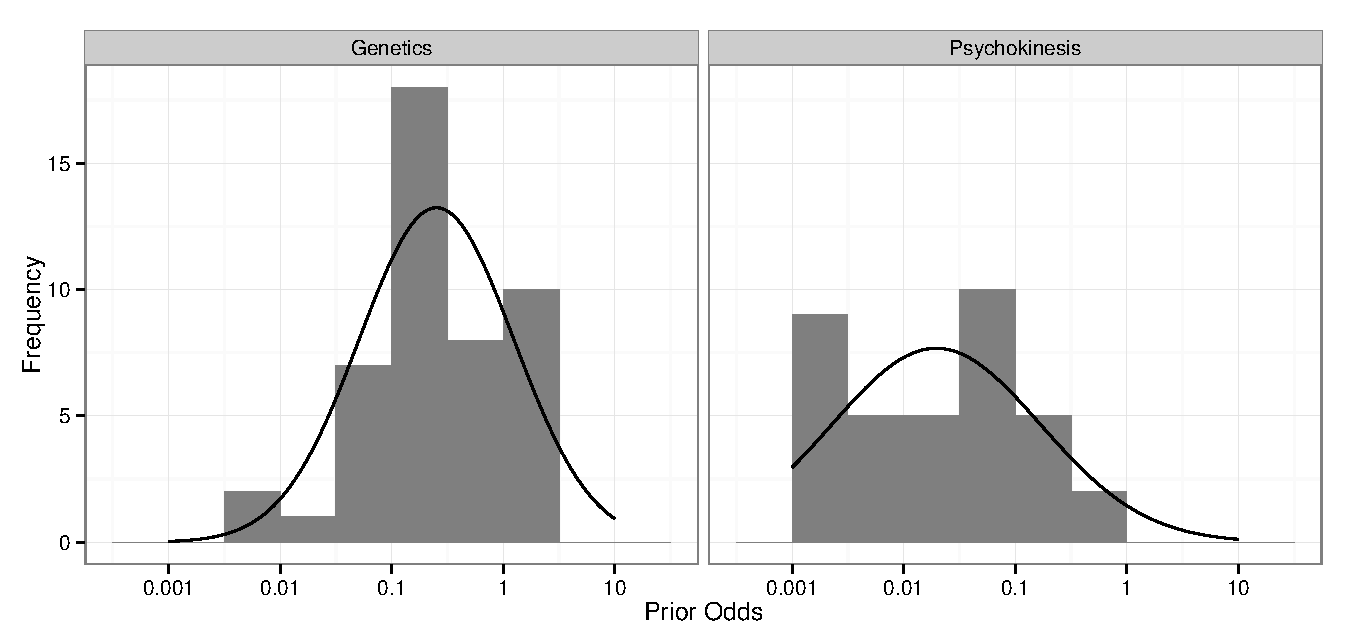
\includegraphics[width=.95\textwidth]{coincidences_figures/priorVariation.pdf}
	\caption{The cover story has a strong influence on the prior probability of an effect. Individual subject distributions over the prior odds vary with condition, with people who saw the {\sc genetics} cover story giving much higher prior odds of a real effect. Even within condition, however, people vary a great deal in their prior beliefs.}
	\label{fig:coverstory}
\end{figure}

\begin{figure}[]
	\centering
	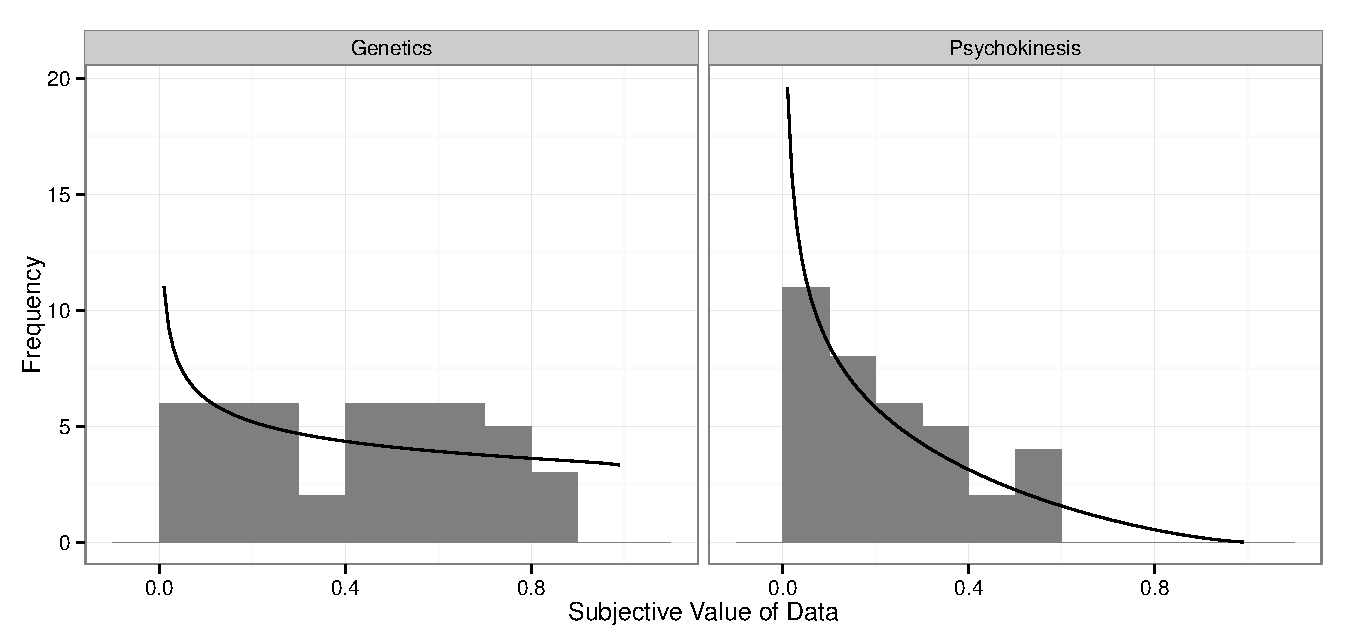
\includegraphics[width=.95\textwidth]{coincidences_figures/likelihoodVariation.pdf}
	\caption{The cover story has an influence on the likelihood. Individual subject distributions over the likelihood also vary with condition, suggesting that people were more distrustful of the evidence in the {\sc psychokinetic} condition: The average subjective value of an observation is 43\% in the {\sc genetics} condition but only 23\% in the {\sc psychokinetic} condition. In both conditions, people acted far more conservatively than the ``optimal'' Bayesian model would predict.}
	\label{fig:coverstory2}
\end{figure}



% numbers extracted from the estimated distributions
%
% posterior mean for the likelihood: 
%    genetics = .43, [ci .33 .53]   %% <- raw subj: .42
%    psychokinesis = .23 [ ci .16 .33 ] %% <- raw subj .22
% posterior mean for the log prior: 
%    genetics = 1:4, [ci 2.3, 6.8]
%    psychokinesis = 1:51 [ci 21, 140]


\subsubsection*{The effect of the cover story manipulation}

The merits of the descriptive approach become more apparent once we revisit the original question that GT1 sought to answer using their experiment. In the original paper, they concluded that the cover story influenced people's priors. In our re-analysis using the descriptive model we replicate this finding, and in fact are able to extend it slightly by quantifying the magnitude of the effect: In the {\sc genetics} condition, the average prior $\phi$ used by subjects corresponded to a 4:1 prior bias in favor of the null hypothesis (i.e, no effect), whereas in the {\sc psychokinesis} condition the bias to prefer the null was 51:1 on average. The 95\% credible intervals for these are $[2.3, 6.8]$ and $[21,140]$ respectively, which do not overlap: This indicates that the effect is almost certainly genuine. Individual subject distributions over the prior odds are plotted in Figure~\ref{fig:coverstory}. In essence, these results replicate the findings reported by GT1, though they are somewhat more detailed. 

However, in addition to being more detailed, our analysis departs from GT1 in a more fundamental way: The descriptive framework allows us to consider the possibility that the cover story manipulation {\it also} affects the choice of likelihood function. As discussed previously, there is no reason why the prior is the only way people might change their behavior in response to a change in cover story. People may simply be more distrustful of evidence in the {\sc psychokinesis} condition, leading to a shift in the likelihood as well as the prior \cite<e.g.>{Welsh2012}. In fact, when we investigate this with the descriptive model, it is precisely what we find: In both conditions participants tend to be conservative, downgrading the evidentiary value of an observation relative to the behavior of the optimal model. In the {\sc genetics} condition the average subjective value of an observations is inferred to be 43\% of that assumed by the original Bayesian analysis (i.e., average $\theta$ = .43), with a 95\% credible interval of $[.33, .53]$. In the {\sc psychokinesis} condition this drops to 23\% (95\% credible interval: $[.16, .33]$). As before, the disjoint credible intervals imply strong evidence for an effect. The individual subject distributions are plotted in Figure~\ref{fig:coverstory2}.

\subsection*{Discussion}

The original paper by GT1 develops an elegant Bayesian theory about how people integrate prior knowledge with statistical evidence in order to discriminate mere coincidences from meaningful discoveries, one that is not restricted to the particular special case that we reanalyze here. There is much to like about the theory, not least of which is the demonstration that people {\it do} integrate prior knowledge with statistical evidence when evaluating data. Even so, the original rational analysis makes theoretical claims that go beyond the assertion that people integrate background knowledge with statistical evidence: GT1 claim that the manner in which people do so is ``appropriate'', and that the only source of ``irrationality'' that people bring to these tasks is via miscalibrated priors. In retrospect it appears that these claims are not justified when we look at individual subject data. Absent any compelling justification why people {\it ought} to have used likelihoods that no statistician would ever apply to the results of a genetic engineering study, it is not at all clear that we should conclude that people integrate prior knowledge with statistical evidence in an appropriate fashion, much less an optimal one. Normative claims about human cognition do not seem to be licensed by these data. 

Although it turns out that people's behavior systematically deviates from the normative standard set by the optimal Bayesian model, those deviations turn out to be interesting in a way that is naturally captured by the descriptive Bayesian model. In other words, the successes of the descriptive model go beyond mere data fitting: At the end of our analysis we arrived at a nuanced psychological understanding of the task that was not possible with the optimal model alone. As experimenters, we did not know {\it a priori} whether different likelihood functions would be needed to capture individual differences in human judgments, but we were able to learn the answer from participant responses (they are). We did not know if individual subjects would be consistent with our model (mostly yes), nor whether they would be consistent with the original model (sometimes yes). We suspected that background knowledge would affect people's prior biases (it did), but we did not know if it would also shape people's willingness to have those initial beliefs modified by evidence (it did). Overall, the descriptive approach yields a more detailed and nuanced description of how people evaluate evidence. We can no longer conclude, as did GT1, that people reason optimally but bring different priors to different situations; it now appears that people not only have different pre-existing beliefs, but they also update their beliefs conservatively (and that the extent of this conservatism is sensitive to the situation). This finding opens up many psychologically interesting questions about why and when people do (or should) conservatively update their beliefs---questions that are not easily explored with a rational Bayesian analysis.

As a final point, it is important to clarify that we are not claiming that GT1 simply failed to look at individual differences. Rather, we argue that focusing on questions about optimality tends to discourage researchers from reporting or discussing them. When people differ in substantive ways from one another, it is always possible to imagine that each person is responding in a fashion that is optimal conditional on the particular experiences a person has had, but it is very difficult to provide evidence for such a claim.\footnote{It is also worth noting that one could apply a notion of {\it constrained} optimality to look at individual differences---but only to the extent that those individual differences can be tied to the constraints. For instance, if researchers were trying to argue that are optimal on some task conditional on their limited memory, it would be natural to measure people’s memory and determine if differences in performance on that task were related to their memory capacity. But GT1 were not making any claims like this; they were investigating the issue of whether people {\it in general} were optimal on this task---and with that viewpoint, it was natural to not even think of investigating individual differences.} Indeed, if the researcher's theory supplies only a single notion of optimality, then the mere existence of individual differences is at odds with the claim that human behavior on the task is optimal. As a consequence, while it is not impossible to reconcile individual differences with an optimality claim, in practice it can be awkward to do so. As such Bayesian optimal modeling imposes a theoretical straightjacket that discourages consideration of individual differences. By making the theoretical shift to a descriptive Bayesian approach, the exploration of individual differences becomes possible because the constraints imposed by claims of optimality are removed. Taking these various considerations together, it is clear that in this instance a descriptive approach to Bayesian cognitive modelling provides a better account of human performance than an optimal model, and sheds more light on how people solve the underlying inference problem. 





